% !TEX root = DesignDocument.tex


\chapter{Prototypes}

\begin{comment}This chapter is for recording each prototype developed.  It is a historical record of what you accomplished in 464/465.   This should be organized according to Sprints.  It should have the basic description of the sprint deliverable and what was accomplished.  Screen shots, photos, captures from video, etc should be used. 
\end{comment} 

\section{Sprint 1 Prototype}
\subsection{Deliverables}
\begin{itemize}
\item Software Contract
\item Sprint Report 1
\item Hardware Decision
\end{itemize}

\subsection{Backlog}
\subsection*{Azure}
\begin{itemize}
\item Set up Azure
\item Create Azure database
\item User Authentication
\item App Communication
\end{itemize}

\subsection*{Web Application}
\begin{itemize}
\item Create Web App project
\item Upload Web App project to Azure
\item Create website login screen
\item Communicate with Azure
\item Create schedule templates
\item \#14: Update Web App Homepage 
\item \#20: Create Dashboard View
\item \#21: Revamp Login and Register Web App Pages 
\item \#30 Web App - Open calendar framework JSON events
\item \#31 Web App - Connect calendar event creation to database
\item \#33 Web App - Load events from database when navigating to dashboard controller
\item \#34: Web App - Remove authorization code
\item \#35 Create Unit test projects for both the web applications and web API projects
\item \#37 Web App (TEAM) - Create wireframe for design
\item Code the user interface according to wireframes
\item \#58 Web App - Add code to insert calendar events into database
\item \#59 Web App - Grab JSON from calendar framework
\item \#60 Web App - Load events from database
\item Create distinguished views for each type of user
\item Role based detection
\item Registration process
\item Database table integration and referencing
\item Repetition to generate repeated calendar events
\item Handle temporary canceled events
\end{itemize}

\subsection*{Web API}
\begin{itemize}
\item Create Web API project
\item Update Web API project to Azure
\item Model Location
\item Repository Layer
\item Serialize data
\item Migration on database
\item Create API endpoints for moving schedule data back and forth
\item \#24 Web API - Create Professor Model
\item \#25 Web API - Create Office Personnel Model
\item \#26 Web API - Create Calendar Event Model
\item \#27 Web API - Model Location
\item \#28 Web API - Create GetCalendarEvent endpoint
\item \#29 Web API - Create GetCalendarEvents endpoint
\item \#32 Web API - Create SaveCalendarEvents endpoint
\item \#35 Create Unit test projects for both the web applications and web API projects
\item \#41 Web API - Repository Layer
\item \#43 Web API - Serialize data
\item \#61 Web API - Fix Models
\item \#62 Web API - Create GetCalendarEventsByOwner endpoint
\item \#64 Web API - Create GetCalendarEventsByRoom
\item \#67 Web API - Display options endpoints
\item \#68 Web API - Create GetCalendarEventsByRange
\item \#69 Web API - Model updates
\item Testing
\end{itemize}

\subsection*{Tablet Application}
\begin{itemize}
\item Design and create splash screen
\item Enable tablet to connect to Azure
\item Create communication class
\item Display a message on tablet screen
\item Display schedule on tablet	
\item Learn XamarinLearn Xamarin\footnote{See Appendix \ref{XamarinAppendix}\label{note4}}
\item Create Xamarin tablet application with a login page\textsuperscript{\ref{note4}}
\item \#17 Create Xamarin Tablet App
\item \#18 Tablet App - Android Kiosk Mode for Tablet App
\item \#19 Second Tablet App View
\item \#36 Tablet App - Create Calendar View
\item \#38 Tablet App (TEAM) - Create wireframe for tablet app
\item Code the user interface according to wireframes
\item \#39 Tablet App - Create communications class
\item \#40 Tablet App - Create a way to display JSON calendar events
\item \#42 Tablet App - Move Tablet Code
\item \#53 Android calendar framework JSON function
\item Create pop-up window with description
\item Modify week view class open source
\item Added synchronization button
\item Implement continuous synchronization
\item Create login page
\item Add a view to select calendar based on faculty or room
\item Token authentication
\item GUI modifications
\item Handle temporary canceled events
\item Testing
\end{itemize}

\subsection*{Miscellaneous}
\begin{itemize}
\item Logo
\item Research Tablet vs Odroid Options
\item Connect Visual Studio to Azure
\item Look into networking for tablets
\item Look into a pre-built calendar framework for displaying calendar events
\item Create middleman project
\item Make sure system is very secure
\item \#54 Understand how event ownership works
\end{itemize}

\subsection{Success/Fail}
Our success was understanding and combining the visions of the clients.


\section{Sprint 2 Prototype}
\subsection{Web Application}
\subsubsection{Deliverable}
By the end of sprint 2, we wanted to have an ASP.NET Web App project hosted in Azure and accessible via a URL. In addition, we also wanted to be able to navigate to a "dashboard" view on the web app site that would allow a user to see a weekly display of calendar events.
\subsubsection{Backlog}
\begin{itemize}
\item Upload Web App project to Azure
\item Create website login screen
\item Communicate with Azure
\item Create schedule templates
\item \#14: Update Web App Homepage - For this issue, the web app homepage was updated from the stock web app template to reflect the DoorPanes project. The text and the site colors were updated under this issue.
\item \#20: Create Dashboard View - For this issue, a dashboard controller and a dashboard view were added to the web app project. Once this was done, a user could navigate to the dashboard controller and see a listing of calendar events.
\item \#21: Revamp Login and Register Web App Pages - For this issue, the login page and the register page were updated to reflect the homepage design.
\item \#30 Web App - Open calendar framework JSON events
\item \#31 Web App - Connect calendar event creation to database
\item \#33 Web App - Load events from database when navigating to dashboard controller
\item \#34: Web App - Remove authorization code
\item \#35 Create Unit test projects for both the web applications and web API projects
\item \#37 Web App (TEAM) - Create wireframe for design
\item Code the user interface according to wireframes
\item \#58 Web App - Add code to insert calendar events into database
\item \#59 Web App - Grab JSON from calendar framework
\item \#60 Web App - Load events from database
\item Create distinguished views for each type of user
\item Role based detection
\item Registration process
\item Database table integration and referencing
\item Repetition to generate repeated calendar events
\item Handle temporary canceled events
\end{itemize}


%The items in that were in the backlog for sprint 2 for the Web App were as follows:

%\begin{itemize}
%\item Issue \#14: Update Web App Homepage - For this issue, the web app homepage was updated from the stock web app template to reflect the DoorPanes project. The text and the site colors were updated under this issue.
%\item Issue \#20: Create Dashboard View - For this issue, a dashboard controller and a dashboard view were added to the web app project. Once this was done, a user could navigate to the dashboard controller and see a listing of calendar events.
%\item Issue \#21: Revamp Login and Register Web App Pages - For this issue, the login page and the register page were updated to reflect the homepage design. 
%\end{itemize}

\subsubsection{Success/Fail}
All of the issues pertaining to the web app for sprint 2 were accomplished during Sprint 2.

\subsection{Web API}
\subsubsection{Deliverable}
The Web API project was created.
\subsubsection{Backlog}
\begin{itemize}
\item Create Web API project
\item Update Web API project to Azure
\item Model Location
\item Repository Layer
\item Serialize data
\item Migration on database
\item Create API endpoints for moving schedule data back and forth
\item \#16: Create MVC models
\item \#22: Create API endpoints
\item \#24 Web API - Create Professor Model
\item \#25 Web API - Create Office Personnel Model
\item \#26 Web API - Create Calendar Event Model
\item \#27 Web API - Model Location
\item \#28 Web API - Create GetCalendarEvent endpoint
\item \#29 Web API - Create GetCalendarEvents endpoint
\item \#32 Web API - Create SaveCalendarEvents endpoint
\item \#35 Create Unit test projects for both the web applications and web API projects
\item \#41 Web API - Repository Layer
\item \#43 Web API - Serialize data
\item \#61 Web API - Fix Models
\item \#62 Web API - Create GetCalendarEventsByOwner endpoint
\item \#64 Web API - Create GetCalendarEventsByRoom
\item \#67 Web API - Display options endpoints
\item \#68 Web API - Create GetCalendarEventsByRange
\item \#69 Web API - Model updates
\item Testing
\end{itemize}

\subsubsection{Success/Fail}
Our success was finally understanding the necessary steps to implement the API models and controllers. Another success was figuring out how the API connected to the database. We failed at getting a good start on the API in this sprint. We also realized we needed to break the backlog down into more specific tasks.

\subsection{Tablet Application}
\subsubsection{Deliverable}
During Sprint 2, our tablet application was being developed using Xamarin. We fell into many issues getting the Xamarin environment to be set up correctly. We were unable to develop a working application during this sprint.  However, our idea for the look of this application is shown in Figure \ref{fig:firstview} and Figure \ref{fig:navdrawer}. 

\begin{figure}
\centering
  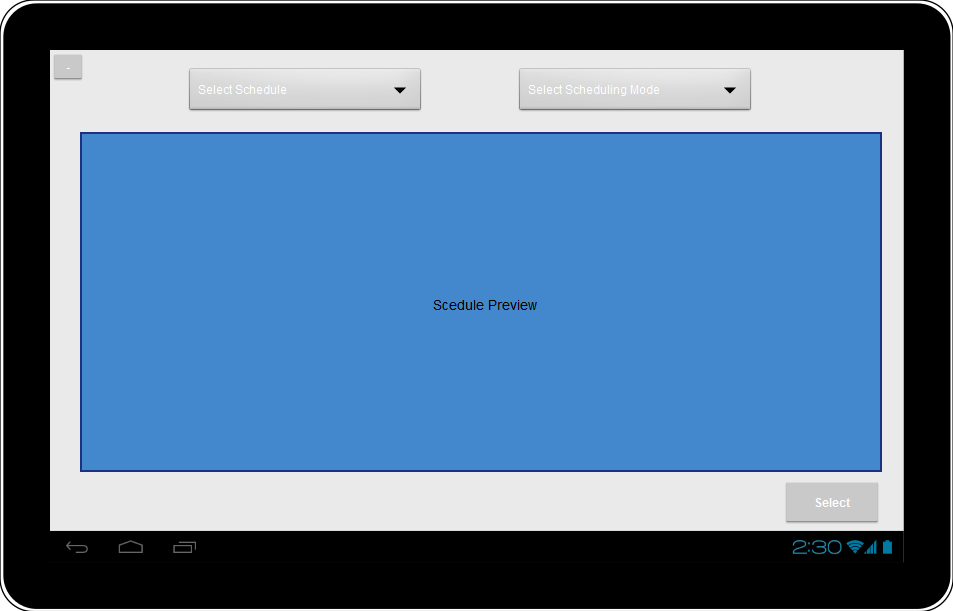
\includegraphics[scale=0.45]{firstview.png}
  \caption{Preview Page}
  \label{fig:firstview}
\end{figure}

\begin{figure}
\centering
  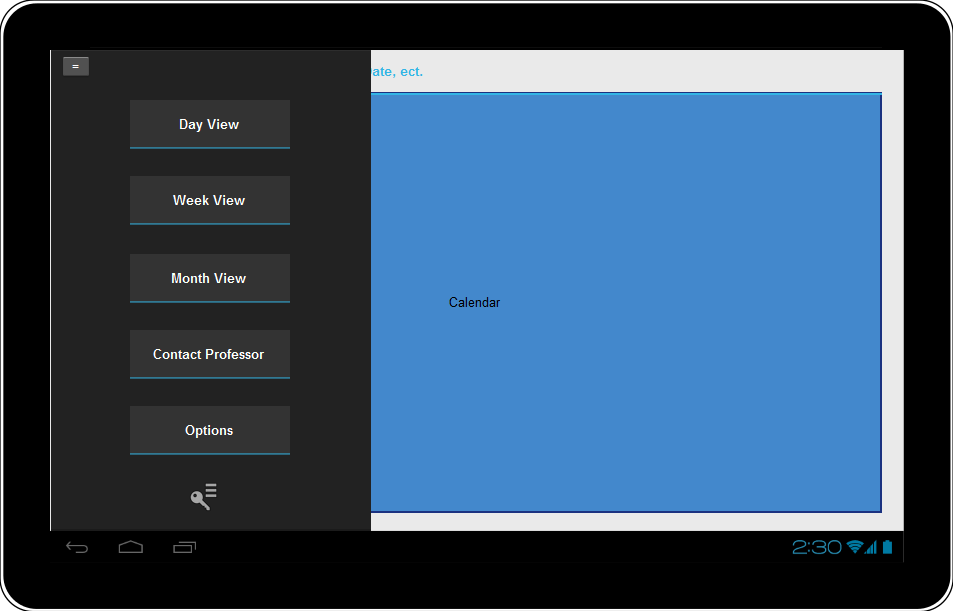
\includegraphics[scale=0.45]{navigationdrawer.png}
  \caption{Dashboard view with navigation drawer expanded}
  \label{fig:navdrawer}
\end{figure}
\subsubsection{Backlog}
\begin{itemize}
\item Design and create splash screen
\item Enable tablet to connect to Azure
\item Display a message on tablet screen
\item Display schedule on tablet	
\item Learn XamarinLearn Xamarin\footnote{See Appendix \ref{XamarinAppendix}\label{note2}}
\item Create Xamarin tablet application with a login page\textsuperscript{\ref{note2}}
\item \#17 Create Xamarin Tablet App
\item \#18 Tablet App - Android Kiosk Mode for Tablet App
item \#19 Second Tablet App View
\item \#36 Tablet App - Create Calendar View
\item \#38 Tablet App (TEAM) - Create wireframe for tablet app
\item Code the user interface according to wireframes
\item \#39 Tablet App - Create communications class
\item \#40 Tablet App - Create a way to display JSON calendar events
\item \#42 Tablet App - Move Tablet Code
\item \#53 Android calendar framework JSON function
\item Create pop-up window with description
\item Modify week view class open source
\item Added synchronization button
\item Implement continuous synchronization
\item Create login page
\item Add a view to select calendar based on faculty or room
\item Token authentication
\item GUI modifications
\item Handle temporary canceled events
\item Testing
\end{itemize}

\subsubsection{Success/Fail}
At the end of this sprint it was decide we were no longer going to use Xamarin to develop our tablet application.  All future development will be done using Android Studio.  The little work that was accomplished in Xamarin will be transferred to native Android.

\subsection*{Miscellaneous Backlog}
\begin{itemize}
\item Logo
\item Connect Visual Studio to Azure
\item Look into networking for tablets
\item Create middleman project
\item Make sure system is very secure
\item \#54 Understand how event ownership works
\end{itemize}

\section{Sprint 3 Prototype}
\subsection{Web Application}
\subsubsection{Deliverable}
By the end of sprint 3, we wanted to have the ability to add and remove calendar events from the dashboard controller and have the changes made to the dashboard calender event view persist when a user closed the browser window/tab.
\subsubsection{Backlog}
\begin{itemize}
\item \#30 Web App  - Open calendar framework JSON events. For this issue, we needed to understand how the open source calendar framework we were using stored JSON calendar events.
\item \#31 Web App - Connect calendar event creation to database. For this issue, the calendar event creation mechanism in the open source calendar framework needed to be connected to an endpoint that would create a calendar event model and store it in the database.
\item \#33 Web App - Load events from database when navigating to dashboard controller. For this issue, the load event hook in the open source calendar framework needed to be connected to the get calendar events web app endpoint so events could be loaded from the database when the user navigated to the dashboard page.
\item \#34: Web App - Remove authorization code. For this issue, the authorization code was removed from the web app so data-flow development could happen without needing to worry about being authorized yet. The authorization code will be added in at a later date.
\item \#35 Create Unit test projects for both the web applications and web API projects
\item \#37 Web App (TEAM) - Create wireframe for design
\item Code the user interface according to wireframes
\item \#58 Web App - Add code to insert calendar events into database
\item \#59 Web App - Grab JSON from calendar framework
\item \#60 Web App - Load events from database
\item Create distinguished views for each type of user
\item Role based detection
\item Registration process
\item Database table integration and referencing
\item Repetition to generate repeated calendar events
\item Handle temporary canceled events
\end{itemize}

%The issues that were in the backlog for sprint 3 for the Web App were as follows:

%\begin{itemize}
%\item Issue \#30: Web App - Open calendar framework JSON events. For this issue, we needed to understand how the open source calendar framework we were using stored JSON calendar events.
%\item Issue \#31: Web App - Connect calendar event creation to database. For this issue, the calendar event creation mechanism in the open source calendar framework needed to be connected to an endpoint that would create a calendar event model and store it in the database.
%\item Issue \#33: Web App - Load events from database when navigating to dashboard controller. For this issue, the load event hook in the open source calendar framework needed to be connected to the get calendar events web app endpoint so events could be loaded from the database when the user navigated to the dashboard page.
%\item Issue \#34: Web App - Remove authorization code. For this issue, the authorization code was removed from the web app so data-flow development could happen without needing to worry about being authorized yet. The authorization code will be added in at a later date.
%\end{itemize}

\subsubsection{Success/Fail}
Due to struggles with the API endpoint creation and major issues with the tablet app, the only issue that was resolved was Issue \#30 (understanding the JSON event storage in the open source calendar framework). The remaining issues will have to be moved to a later sprint.

\subsection{Web API}
\subsubsection{Deliverable}
The following was created and implemented in this sprint:
Endpoints
\begin{itemize}
\item Get Calendar Events By Owner
\item Get Calendar Events
\item Save Calendar Events
\end{itemize}
Models
\begin{itemize}
\item Office Personnel Model
\item Instructor Model
\item Person Model
\item Event Model
\end{itemize}
\subsubsection{Backlog}
\begin{itemize}
\item Create Web API project
\item Update Web API project to Azure
\item Model Location
\item Repository Layer
\item Migration on database
\item Create API endpoints for moving schedule data back and forth
\item \#24 Web API - Create Professor Model
\item \#25 Web API - Create Office Personnel Model
\item \#26 Web API - Create Calendar Event Model
\item \#27 Web API - Model Location
\item \#28 Web API - Create GetCalendarEvent endpoint
\item \#29 Web API - Create GetCalendarEvents endpoint
\item \#32 Web API - Create SaveCalendarEvents endpoint
\item \#35 Create Unit test projects for both the web applications and web API projects
\item \#41 Web API - Repository Layer
\item \#43 Web API - Serialize data
\item \#61 Web API - Fix Models
\item \#62 Web API - Create GetCalendarEventsByOwner endpoint
\item \#64 Web API - Create GetCalendarEventsByRoom
\item \#67 Web API - Display options endpoints
\item \#68 Web API - Create GetCalendarEventsByRange
\item \#69 Web API - Model updates
\item Testing
\end{itemize}

\subsubsection{Success/Fail}
Our success in this sprint for the web API component was that everything in the backlog was completed or nearly  completed.

\subsection{Tablet Application}
\subsubsection{Deliverable}
Once switched over to native Android, development went a lot smoother.  A wireframe model was developed including a good portion of the features needed for our finished product.  The screenshots of our prototype are shown starting with Figure ~\ref{fig:loginscreen}.  One upgrade in Android Studio as opposed to Xamarin, is the implementation of activities.  An activity is a single, focused thing the user can do.  The use of activites allows for the user to switch between screen views, rotate the tablet, switch to another application, and the state of the app is saved and restarted when any said action occurs.  It was more difficult to create these activites using Xamarin.  



\begin{figure}
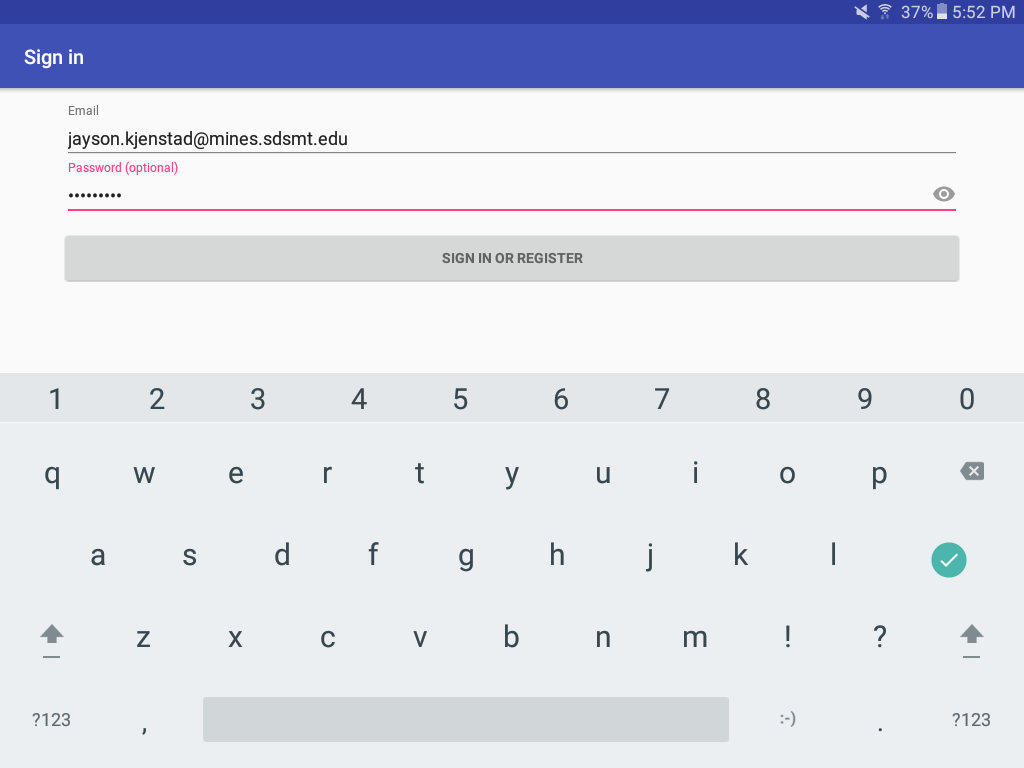
\includegraphics[scale=0.45]{loginscreen.png}
\caption{Login screen}
\label{fig:loginscreen}
\end{figure}

\begin{figure}
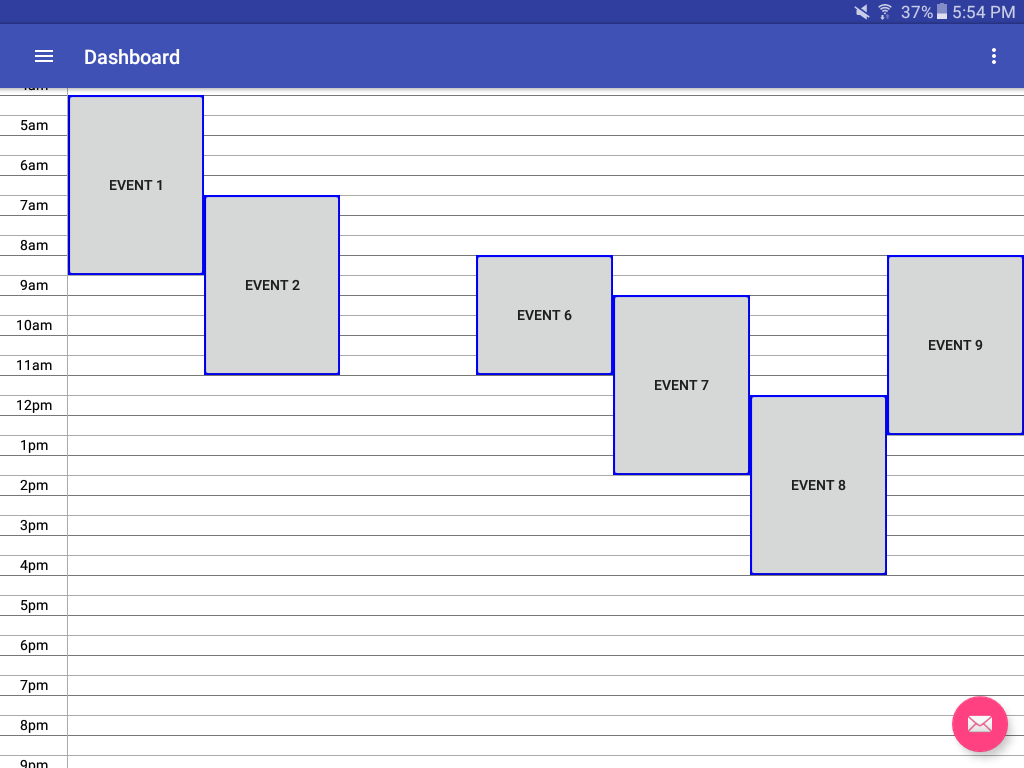
\includegraphics[scale=0.45]{calendarview.png}
\caption{Calendar view with events}
\label{fig:calendar}
\end{figure}

\begin{figure}
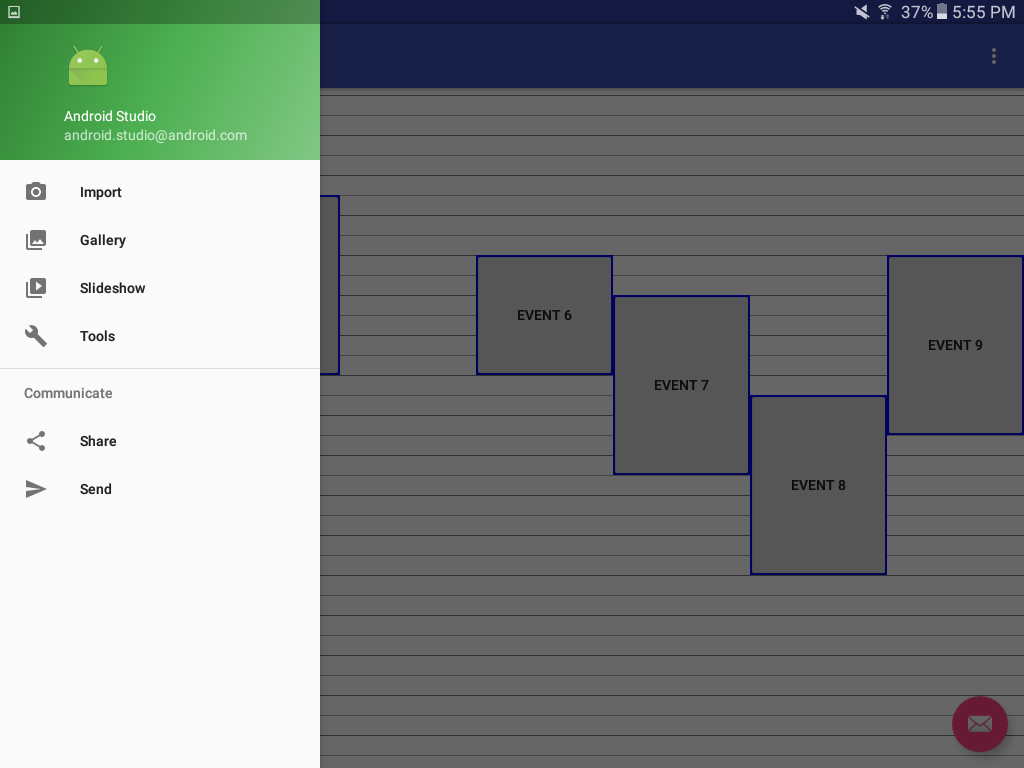
\includegraphics[scale=0.45]
{navigation.png}
\caption{Dashboard view with navigation drawer expanded}
\label{fig:nav}
\end{figure}

\subsubsection{Backlog}
\begin{itemize}
\item Design and create splash screen
\item Enable tablet to connect to Azure
\item Display a message on tablet screen
\item Display schedule on tablet	
\item Learn XamarinLearn Xamarin\footnote{See Appendix \ref{XamarinAppendix}\label{note3}}
\item Create Xamarin tablet application with a login page\textsuperscript{\ref{note3}}
\item \#18 Tablet App - Android Kiosk Mode for Tablet App
\item \#36 Tablet App - Create Calendar View
\item \#38 Tablet App (TEAM) - Create wireframe for tablet app
\item Code the user interface according to wireframes
\item \#39 Tablet App - Create communications class
\item \#40 Tablet App - Create a way to display JSON calendar events
\item \#42 Tablet App - Move Tablet Code
\item \#53 Android calendar framework JSON function
\item Create pop-up window with description
\item Modify week view class open source
\item Added synchronization button
\item Implement continuous synchronization
\item Create login page
\item Add a view to select calendar based on faculty or room
\item Token authentication
\item GUI modifications
\item Handle temporary canceled events
\item Testing
\end{itemize}

\subsubsection{Success/Fail}
A wireframe for a good portion of the application was created.  A calendar view was created where the JSON calendar events can be displayed as a button on the view.  However, there was no actual integration of the JSON events yet.  That and the communications class will be pushed to our sprint after winter break.

\subsection*{Miscellaneous Backlog}
\begin{itemize}
\item Logo
\item Research Tablet vs Odroid Options
\item Connect Visual Studio to Azure
\item Look into networking for tablets
\item Look into a pre-built calendar framework for displaying calendar events
\item Create middleman project
\item Make sure system is very secure
\item \#54 Understand how event ownership works
\end{itemize}

\section{Sprint 4 Prototype}

\subsection{Web Application}
\subsubsection{Deliverable}
The following were delivered for this sprint:
\begin{itemize}
\item Load events from database
\item Connect web application database to Azure
\item Created middle man project for web application and web API to share
\item Display calendar events on the calendar framework on the web application
\end{itemize}

\subsubsection{Backlog}
The backlog for the web app is the following:
\begin{itemize}
\item \#33 Web App - Load events from database when navigating to dashboard controller
\item \#35 Create Unit test projects for both the web applications and web API projects
\item \#37 Web App (TEAM) - Create wireframe for design
\item Code the user interface according to wireframes
\item \#58 Web App - Add code to insert calendar events into database
\item \#59 Web App - Grab JSON from calendar framework
\item \#60 Web App - Load events from database
\item Create distinguished views for each type of user
\item Role based detection
\item Registration process
\item Database table integration and referencing
\item Repetition to generate repeated calendar events
\item Handle temporary canceled events
\end{itemize}

\subsubsection{Success/Fail}
Some items we fell short on during this sprint were understanding database seeding and migrations problems, GUID usage, and database permissions and authorization.

\subsection{Web API}
\subsubsection{Deliverable}
The following were delivered for this sprint:
\begin{itemize}
\item Return actual JSON from web API endpoints
\item Updated getByOwner endpoint
\item Updated web API models
\item Understand GUID principles
\end{itemize}

\subsubsection{Backlog}
The backlog for the web API is the following:
\begin{itemize}
\item Repository Layer
\item Migration on database
\item \#35 Create Unit test projects for both the web applications and web API projects
\item \#41 Web API - Repository Layer
\item \#43 Web API - Serialize data
\item \#61 Web API - Fix Models
\item \#62 Web API - Create GetCalendarEventsByOwner endpoint
\item \#64 Web API - Create GetCalendarEventsByRoom
\item \#67 Web API - Display options endpoints
\item \#68 Web API - Create GetCalendarEventsByRange
\item \#69 Web API - Model updates
\item Testing
\end{itemize}

\subsubsection{Success/Fail}
Some setbacks we encountered during this sprint were understanding database seeding and migrations problems (didn't understand how they worked), GUID usage, and database permissions and authorization.

\subsection{Tablet Application}
\subsubsection{Deliverable}
The following were delivered for this sprint:
\begin{itemize}
\item Making a get request to an Azure server from the tablet application and getting JSON returned
\item Displaying JSON calendar events on the tablet application screen
\item Understand tablet class layout
\end{itemize}

\subsubsection{Backlog}
\begin{itemize}
\item Enable tablet to connect to Azure
\item Display a message on tablet screen
\item Display schedule on tablet	
\item \#18 Tablet App - Android Kiosk Mode for Tablet App
\item \#36 Tablet App - Create Calendar View
\item \#38 Tablet App (TEAM) - Create wireframe for tablet app
\item Code the user interface according to wireframes
\item \#39 Tablet App - Create communications class
\item \#40 Tablet App - Create a way to display JSON calendar events
\item \#53 Android calendar framework JSON function
\item Create pop-up window with description
\item Modify week view class open source
\item Added synchronization button
\item Token authentication
\item GUI modifications
\item Handle temporary canceled events
\item Testing
\end{itemize}

\subsubsection{Success/Fail}
One setback for the tablet application was the amount of time it took understanding and working out retrofit requests.

\subsection*{Miscellaneous Backlog}
\begin{itemize}
\item Logo
\item Look into networking for tablets
\item Make sure system is very secure
\item \#54 Understand how event ownership works
\end{itemize} 

\section{Sprint 5 Prototype}
\subsection{Web Application}

\subsubsection{Deliverable}
The following were delivered for this sprint:
\begin{itemize}
\item Calendar event creation
\item Partially unit tested
\item Save events
\end{itemize}
\subsubsection{Backlog}
\begin{itemize}
\item \#33 Web App - Load events from database when navigating to dashboard controller
\item \#35 Create Unit test projects for both the web applications and web API projects
\item \#37 Web App (TEAM) - Create wireframe for design
\item Code the user interface according to wireframes
\item \#58 Web App - Add code to insert calendar events into database
\item \#59 Web App - Grab JSON from calendar framework
\item \#60 Web App - Load events from database
\item Create distinguished views for each type of user
\item Role based detection
\item Registration process
\item Database table integration and referencing
\item Repetition to generate repeated calendar events
\item Handle temporary canceled events
\end{itemize}

\subsection{Web API}
\subsubsection{Deliverable}
The following were delivered for this sprint:
\begin{itemize}
\item Unit Tested the current endpoints
\item Create Get calendar events by room
\end{itemize}

\subsubsection{Backlog}
\begin{itemize}
\item Repository Layer
\item Migration on database
\item \#35 Create Unit test projects for both the web applications and web API projects
\item \#64 Web API - Create GetCalendarEventsByRoom
\item \#67 Web API - Display options endpoints
\item \#68 Web API - Create GetCalendarEventsByRange
\item \#69 Web API - Model updates
\item Testing
\end{itemize}

\subsubsection{Success/Fail}
The GetCalendarEventsByRange endpoint was delayed and pushed to the final sprint.

\subsection{Tablet Application}
\subsubsection{Deliverable}
The following were delivered for this sprint:
\begin{itemize}
\item Calendar event synchronization
\item GUI testing
\item Unit test for login screen
\item GUI modifications
\item Calendar description window
\end{itemize}
\subsubsection{Backlog}
\begin{itemize}
\item \#18 Tablet App - Android Kiosk Mode for Tablet App
\item Create pop-up window with description
\item Modify week view class open source
\item Implement continuous synchronization
\item Add a view to select calendar based on faculty or room
\item Token authentication
\item Handle temporary canceled events
\item Testing
\end{itemize}

\subsubsection{Success/Fail}
A setback for the tablet application this sprint was testing JSON responses

\subsection*{Miscellaneous Backlog}
\begin{itemize}
\item Logo
\item Look into networking for tablets
\item Make sure system is very secure
\item \#54 Understand how event ownership works
\end{itemize}

\section{Sprint 6 Prototype}
\subsection{Web Application}
\subsubsection{Deliverable}
The following were delivered for this sprint:
\begin{itemize}
\item Database table integration
\item Database table referencing
\item Person detection based on roles
\item Registration process
\item Different login views based on users
\item Repetition calendar event auto generated implemented but not used
\end{itemize}
\subsubsection{Backlog}
\begin{itemize}
\item Create distinguished views for each type of user
\item Role based detection
\item Registration process
\item Database table integration and referencing
\item Repetition to generate repeated calendar events
\item Handle temporary canceled events
\end{itemize}

\subsubsection{Success/Fail}
During this sprint JavaScript was used often for the continuing development of the web application. Therefore, learning more JavaScript was needed, slowing down progress.

\subsection{Web API}
\subsubsection{Deliverable}
The following were delivered for this sprint:
\begin{itemize}
\item Displays options for endpoint parameters
\item Created Get calendar events by range for room
\item Created Get calendar events by range for owner
\item Room table created
\item Updated models
\item Login and register enabled
\end{itemize}

\subsubsection{Backlog}
\begin{itemize}
\item Migration on database
\item \#67 Web API - Display options endpoints
\item \#68 Web API - Create GetCalendarEventsByRange
\item \#69 Web API - Model updates
\item Testing
\end{itemize}

\subsection{Tablet Application}
\subsubsection{Deliverable}
The following were delivered for this sprint:
\begin{itemize}
\item Added a view to select calendar based on faculty or room
\item Token authentication
\item GUI modifications
\end{itemize}
\subsubsection{Backlog}
\begin{itemize}
\item \#18 Tablet App - Android Kiosk Mode for Tablet App
\item Token authentication
\item Handle temporary canceled events
\end{itemize}

\subsubsection{Success/Fail}
The tablet application had a few hardware issues. 

\subsection*{Miscellaneous Backlog}
\begin{itemize}
\item Logo
\item Look into networking for tablets
\item Make sure system is very secure
\end{itemize}

\section{Final Prototype}

\subsection{Web APP}
The final prototype for the web application includes the ability to sign is as multiple users (instructors, staff, and students all have their own unique views). The final prototype also introduced the ability for staff members to add and view events for multiple rooms. Canceling events was also added in the final prototype. Other additional changes for this final prototype include setup and registration changes to indicate what role the person will be in when they sign up, JavaScript code refactoring and debugging, and calendar model changes to increase data flow flexibility. No major user interface changes were made other than slight HTML element tweaks to show the different views for the different roles. The final UI views for what the interface looks like can be viewed in the user document section of this document. 

\subsection{Web API}
The final prototype for the web API has several endpoints that are working correctly. The endpoints retrieve, save and delete events. The endpoints that get calendar events from the database have specifications except when retrieving all the events stored. A user can get calendar events based on the owner, room, and/or the semester. The API also has endpoints to return all the rooms and owners in the database. The controllers we wrote for the web API are 98\% unit tested

\subsection{Tablet App}
The final prototype for the tablet application has three main parts: login page, calendar select page, and the dashboard view.  The application starts at the login page where the user can enter in credentials made in the web application.  

\begin{figure}
  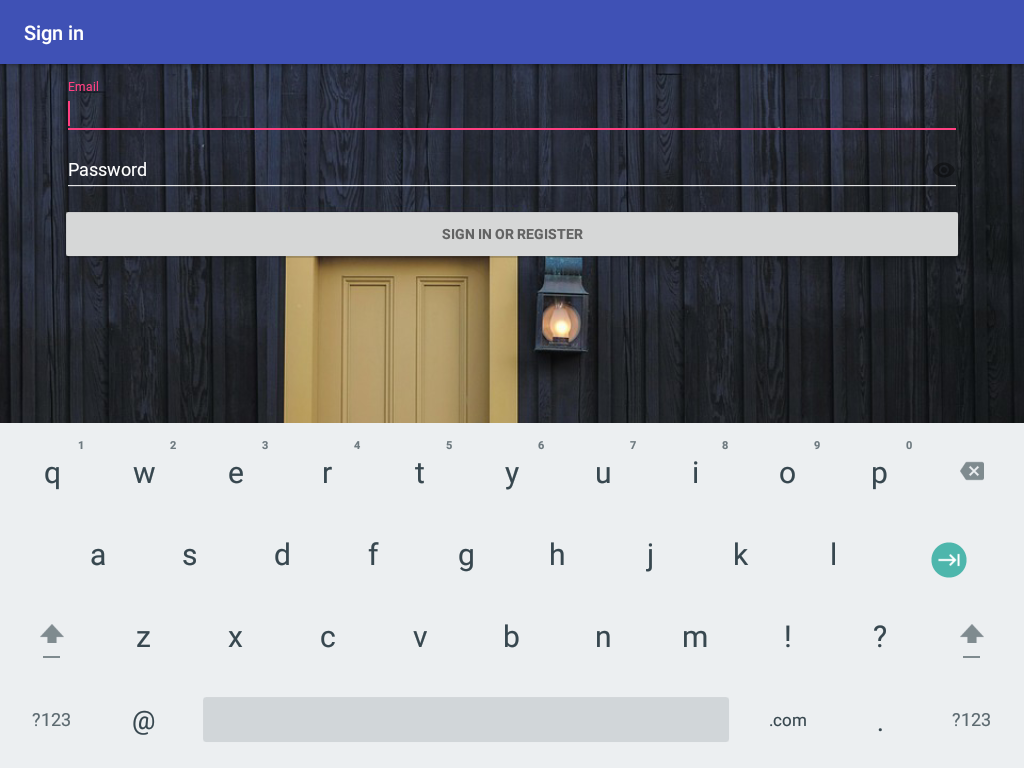
\includegraphics[scale=0.45]{login_final.png}
  \caption{Log in page for tablet application}
  \label{loginfinal}
\end{figure}

The page can be seen in Figure \ref{loginfinal}. On this page, the inputted credentials will be used in an API POST call.  If the password and the username match, a token is sent back in the response body.  This token needs to be used with all other API calls.  After a user logs in, the tablet shows the calendar selection view.  A list of all of the room and faculty schedules from the database are displayed in a dropdown menu.  Radio buttons switch between faculty and room lists.

\begin{figure}
  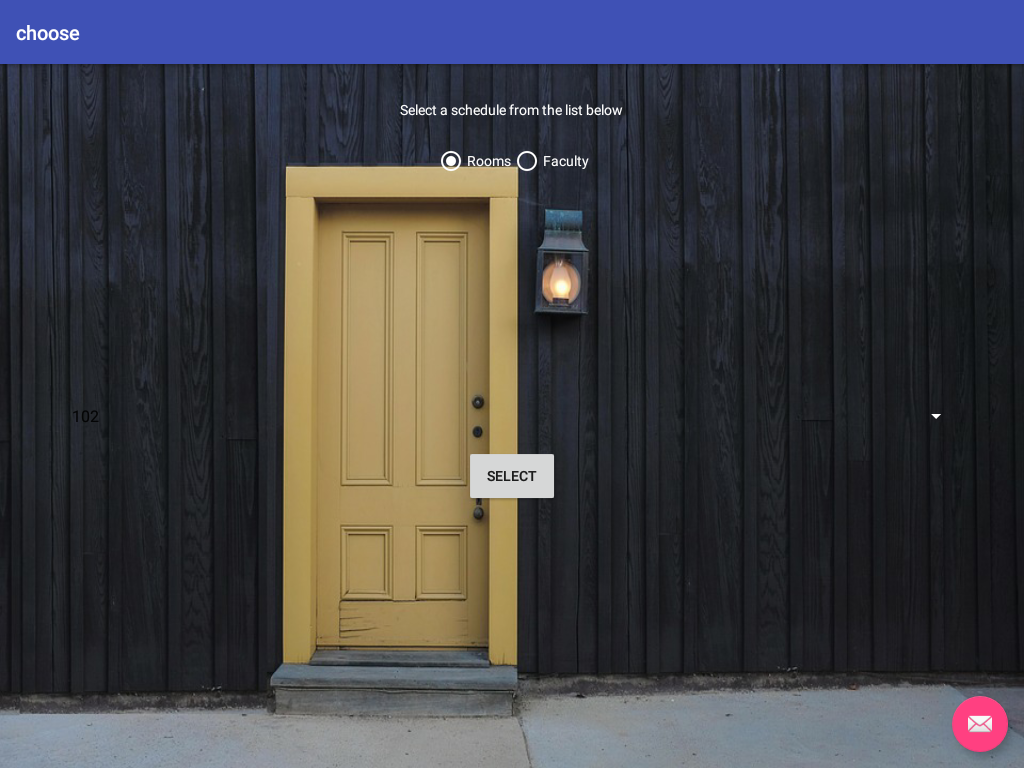
\includegraphics[scale=0.45]{selection_final.png}
  \caption{Calendar selection page for tablet application}
  \label{selectionfinal}
\end{figure}

This page is shown in Figure \ref{selectionfinal}.  After the schedule is selected, the given room or faculty schedule is saved and used for another API call to get all the calendar events.  On the next page, the user must first click the "Sync" button in the navigation drawer.  Once the button is pressed, every 10 seconds a request is sent to get the schedule again to continuously update.  

\begin{figure}
  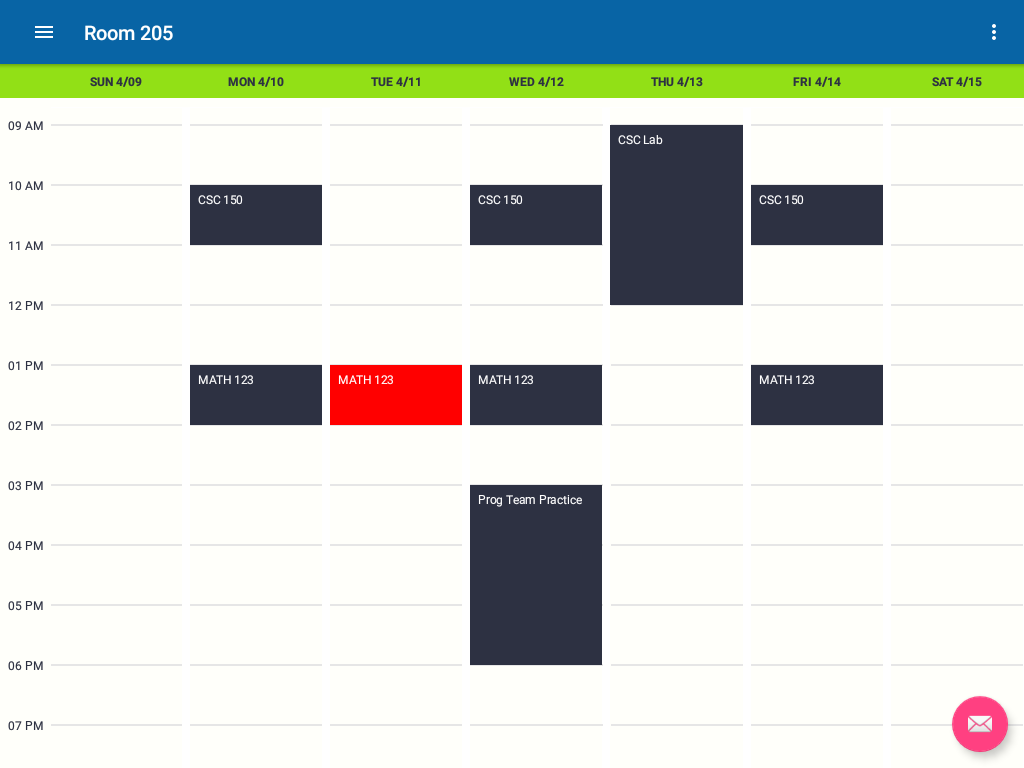
\includegraphics[scale=0.45]{dashboard_final.png}
  \caption{Final calendar view for tablet application}
  \label{dashboardfinal}
\end{figure}

This view can be seen in Figure \ref{dashboardfinal}. As mentioned the tablet will continuously update so it can be mounted and displayed on the proper door!





